\chapter{AI per la visione artificiale}
\begin{wrapfigure}[7]{r}{.45\linewidth}
	\vspace{-.5cm}
	\centering
	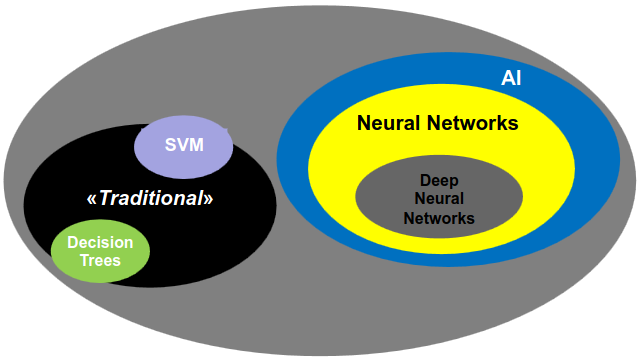
\includegraphics[width=.9\linewidth]{Picture/AI_Classes}
\end{wrapfigure}
L'intelligenza artificiale oggi viene usata in moltissime applicazioni di computer vision e processing di immagini; Le architetture si basano su reti neurali convoluzionali (CNN). In questa trattazione vedremo come si sono evolute le reti neurali partendo dall'idea di percettrone fino ad arrivare alle reti profonde. Per quanto riguarda il metodo di apprendimento ci concentreremo in particolare sull'apprendimento supervisionato.

\section{Percettrone}
Il percettrone è il precursore della moderna AI e cerca di risolvere dei problemi di \textbf{classificazione binaria}. Un problema di questo tipo prevede di riuscire ad etichettare correttamente istanze appartenenti a due classi differenti (esempio: è un cane o un gatto)

\subsection{Funzionamento}
\begin{wrapfigure}[6]{l}{.7\linewidth}
	\vspace{-.2cm}
	\centering
	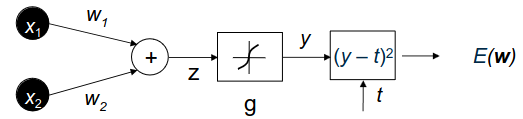
\includegraphics[width=.9\linewidth]{Picture/Perceptron}
\end{wrapfigure}
Nello schema si vede il funzionamento del percettrone, questo calcola una funzione che ha come variabili gli input che riceve e come parametri i pesi $w_i$ degli input. La funzione calcolata è la combinazione lineare degli input pesati e questa serve come input per una funzione di attivazione non lineare, ma differenziabile (tipicamente una \textbf{sigmoide}).
\subsubsection{Aggiornamento dei pesi}\label{sec:stocastic_gradient_descent}
Una volta che è stata calcolata la risposta del percettrone si può calcolare l'errore commesso come scarto quadratico ($E(\vec{w}) = (y - t)^2$) dove $t$ è la classe reale dell'oggetto e può valere 0 o 1. Si può quindi derivare l'errore rispetto al singolo peso con la chain-rule:
\begin{equation}
	\frac{\partial E(\vec{w})}{\partial w_i} = \frac{\partial E}{\partial y} \cdot\frac{\partial y}{\partial z}\cdot \frac{\partial z}{\partial w_i}
\end{equation}
Quindi possiamo aggiornare i pesi considerando il gradiente della funzione errore. Questo metodo si chiama \textbf{stocastic gradient descent}. Passando dall'iterazione $k$ alla $k+1$ possiamo scrivere:
\begin{equation}
	\vec{w}^{k+1} = \vec{w}^k - \eta \nabla_{\vec{w}} E(\vec{w})
\end{equation}
Dove il parametro $\eta$ è detto \textbf{learning rate}, è sempre minore di 1 e influisce su quanto l'errore pesa sull'aggiornamento dei parametri del percettrone.

\subsubsection{Training}
Si inizializzano i pesi casualmente, si calcola l'output per un dato input e si valuta l'errore. Si aggiornano i pesi e si procede in questo modo fino a quando non si esauriscono tutti gli esempi nella classe di training. L'algoritmo
\begin{itemize}
	\item converge se le classi sono linearmente separabili
	\item da come risultato un output binario
\end{itemize}

\section{Multilayer networks}
\begin{wrapfigure}{r}{.45\linewidth}
	\vspace{-.8cm}
	\centering
	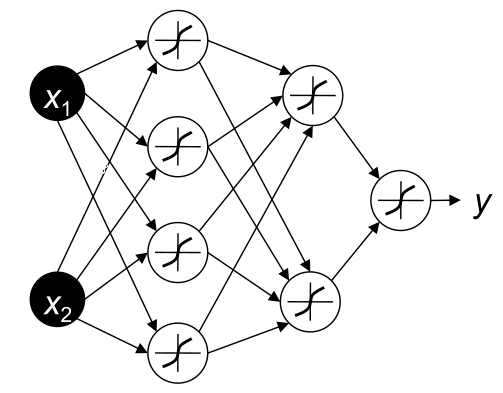
\includegraphics[width=.9\linewidth]{Picture/FCNs}
\end{wrapfigure}
Il singolo neurone permette di classificare classi linearmente separabili. Per poter aumentare la generalità del classificatore si passa alle FCNs (Multilayer Fully Connetted Networks). In queste reti sono presenti uno o più livelli nascosti (hidden), non ci sono cicli e vi è un layer di output.
\newpage
\subsection{Funzionamento}
\begin{wrapfigure}[13]{l}{.63\linewidth}
	\vspace{-.1cm}
	\centering
	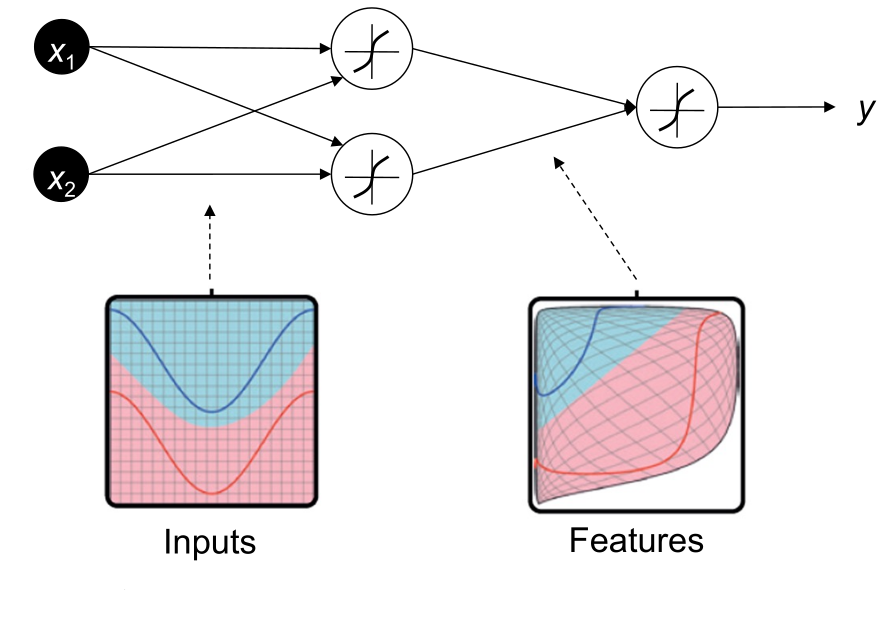
\includegraphics[width=.95\linewidth]{Picture/FCNs_Mapping}
\end{wrapfigure}
I livelli hidden hanno lo scopo di rendere le features linearmente separabili in modo che il livello di output possa operare come descritto prima per il percettrone. L'operazione dei livelli nascosti è quindi una trasformazione dallo spazio degli input allo \textbf{spazio latente} dove si spera che la classificazione sia più semplice. 

Più sono i livelli hidden più è complessa la funzione che si può apprendere per separare le classi.
\subsubsection{Complessità}
La complessità è data dal numero di parametri che devono essere appresi. Per ogni livello il numero di pesi sarà il prodotto tra il numero di input di ogni neurone (+ 1 per il bias)  e il numero di neuroni del layer ovvero il numero di output del layer stesso. Formalmente:
\begin{equation}
	N_{par} = n_{out} \cdot (1+n_in)
\end{equation}

\subsection{Overfitting}
Man mano che si aggiungono livelli e si aumenta la complessità della rete i le funzioni che possono essere apprese diventano sempre più complesse, questo può portare al fenomeno dell'\textbf{overfitting}; che si verifica quando la rete apprende troppo bene i parametri per minimizzare l'errore sul set di training e perde quindi di generalità. Questo fenomeno è evidenziato da un grosso divario tra i punteggi realizzati sul set di training e sul set di validation.

\newpage
\subsubsection{Esempio}
Consideriamo di dover interpolare dei punti con una curva, l'immagine mostra come al variare del numero di gradi di libertà abbiamo 
\begin{multicols}{3}
	\begin{itemize}
		\item underfitting
		\item good fitting
		\item overfitting
	\end{itemize}
\end{multicols}
\begin{center}
	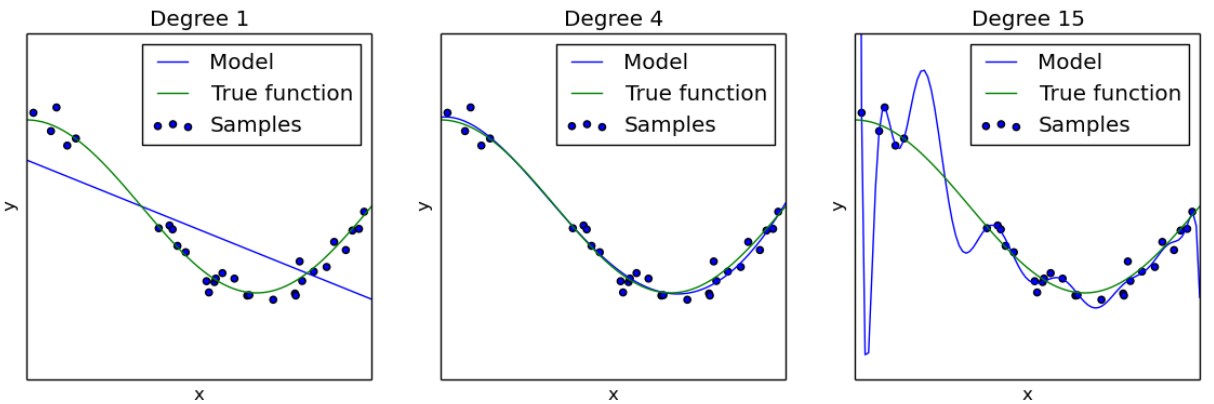
\includegraphics[width=\linewidth]{Picture/Overfitting}
\end{center}
Nell'ultimo caso stiamo fittando il rumore e non i dati.
\subsubsection{Regularization}\label{sec:regularization}
Per impedire l'overfitting si ricorre alla regolarizzazione. Dall'esempio si può immaginare che per far fluttuare così rapidamente la funzione che fa overfitting è necessario che i suoi coefficienti abbiano un \say{grande} valore assoluto. Si cerca di penalizzare le soluzioni con pesi elevati, minimizzando 
\begin{equation}
	J(\vec{w})= E(\vec{w}) + \lambda R(\vec{w}) = E(\vec{w}) + \lambda ||\vec{w}|| ^2
\end{equation}
Dove $R(\vec{w})$ è un fattore di normalizzazione che solitamente si traduce nella norma al quadrato le vettore dei pesi e $\lambda$ è un parametro che normalmente è qualche ordine di grandezza più piccolo del learning rate $\eta$.

\subsection{Multiclass Classification}
Quando abbiamo più di due classi usiamo un livello di output che contiene tanti neuroni quante sono le classi da riconoscere, in questo modo quando incontriamo un oggetto appartenente a una classe si attiva solo il neurone corrispondente e gli altri dovrebbero rimanere spenti. Nella pratica però è raro che si attivi un solo neurone al $100\%$ e gli altri rimangano spenti. Nei casi fortunati avremo un neurone molto attivo e gli altri poco, non è detto però che la somma degli output dei vari neuroni sommi a 1.
\newpage
\subsubsection{Livello Soft-Max}
\begin{wrapfigure}[8]{r}{.6\linewidth}
	\vspace{-.8cm}
	\centering
	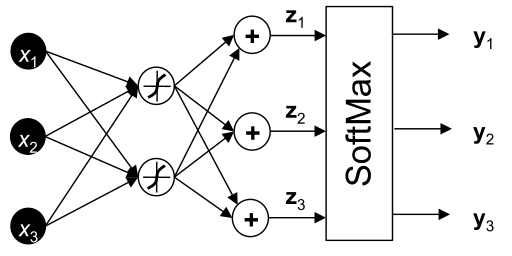
\includegraphics[width=.95\linewidth]{Picture/Multiclass_Soft_Max}
\end{wrapfigure}
Se la somma delle attivazioni dei neuroni non è 1 non possiamo trattarla come una distribuzione di probabilità (PDF). Per risolvere questo problema si aggiunge un livello di normalizzazione che scala gli output dei neuroni e ci assicura di poter trattare il risultato come una PDF.  Per trasformare il risultato dei neuroni in una PDF si usa la formula:
\begin{equation}
	y_i= \sigma(\vec{z})_i = \frac{e^{z_i}}{\sum_{k = 1}^{n} e^{z_k}}  \qquad\text{con } i = 1, 2, \dots, n 
\end{equation}



\subsection{Loss function}
Fino ad ora abbiamo calcolato la funzione d'errore come scarto quadratico (MSE).  Questa politica però ha dei problemi, dato che nella funzione del calcolo dell'errore rientrano anche gli errori dovuti alle classi sbagliate che tendono a spingere $\vec{y}$ verso 0; questo può portare a una distribuzione meno mirata dell'errore.
Definiamo allora la \textbf{Cross Entropy Loss Function} come
\begin{equation}
	L(y, t) = - \sum_i t_i \log(y_i) = - \log(y_{i*})
\end{equation}
Dove $y_{i*}$ è la risposta del neurone associato alla classe corretta e si ottiene dalla sommatoria dato che tutti gli altri $t_i$ valgono 0.

Il risultato di usare la Cross Entropy è:
\begin{itemize}
	\item  l'errore e quindi il gradiente propagato attraverso la rete deriva solo dalla classe corretta $i*$ e ne consegue un aggiornamento dei pesi può mirato;
	\item  all'inizio del training i gradienti sono più grandi e questo porta alla convergenza più rapida dei pesi.
\end{itemize}

\section{Riconoscere immagini}
Ora che abbiamo costruito un sistema in grado di apprendere proviamo a insegnargli a riconoscere le immagini. Il primo tentativo in tal senso è stato fatto per riconoscere le cifre da 0 a 9.

\subsection{LeNet 300}\label{sec:LeNet300}
Il primo compito di classificazione delle immagini consisteva nel riconoscimento di cifre. Queste erano salvate come immagini $28\times28$, in scala di grigi con profondità di 8 bit e contenute in un dataset chiamato \textbf{MNIST}
\subsubsection{Architettura}
\begin{wrapfigure}[6]{r}{.45\linewidth}
	\vspace{-1cm}
	\centering
	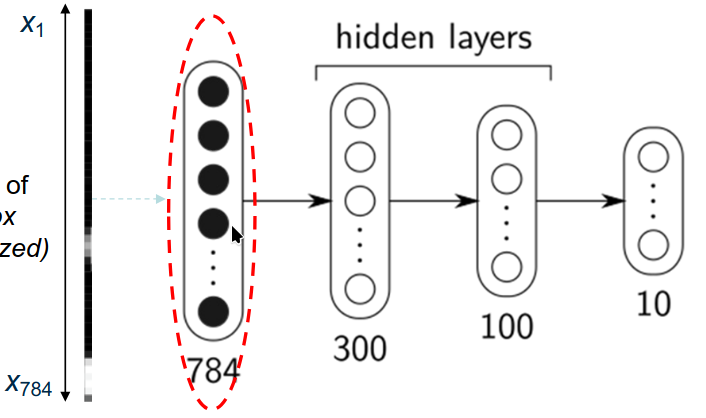
\includegraphics[width=.9\linewidth]{Picture/LeNet_300}
\end{wrapfigure}
La LeNet 300 è una FCN prevede un livello di input costituito da $784$ neuroni, uno per ogni pixel dell'immagine. Ci sono poi 2 livelli hidden costituiti da 300 e 100 neuroni rispettivamente, infine un livello di output costituito da 10 neuroni. La funzione di attivazione del livello di input e dei livelli hidden è una sigmoide, mentre per il livello di output si usa una Soft-Max.
\subsubsection{Pro e contro}
La LeNet migliora le sue performance man mano che si aggiungono livelli hidden e raggiunge, nella configurazione presentata, un tasso di errore del $3.05\%$. 

Aggiungere altri livelli però produrrebbe un grosso incremento della complessità e richiederebbe set di immagini molto grandi per evitare overfitting. Inoltre una FCN non si adatta bene allo scalare delle dimensioni dell'immagine, infatti per ogni pixel è necessario un neurone sul layer di input, questo significa moltissimi neuroni appena si utilizzano immagini di risoluzione maggiore.

\subsection{Un approccio diverso}
Le FCNs prevedono una serializzazione dell'immagine, ogni pixel è mandato a un neurone. Questo però non è come un immagine dovrebbe essere trattata. Le immagini infatti sono caratterizzate da elevata correlazione spaziale, se si serializzano si conserva la correlazione in una sola dimensione.

I filtri, d'altro canto, si comportano così bene sulle immagini perché mantengono la correlazione tra i dati.

Viene quindi naturale pensare di poter applicare l'apprendimento automatico alla costruzione di filtri per riuscire a estrarre le features che più ci interessano per raggiungere il nostro scopo. I pesi dei filtri saranno proprio i parametri che la rete deve apprendere al fine di estrarre le features importanti. Nascono in questo modo le \textbf{reti convoluzionali}.